\documentclass{article}
\usepackage{protools}

\addbibresource{towards.bib}

\setlength\parskip{0.25\baselineskip}

\begin{document}

\ArticleTitle
  {Towards Optical States Of Four Photons}
\ArticleAuthor*
  [0000-0002-5646-6964]
  {Jan Provazn\'{i}k}
  {provaznik@optics.upol.cz}
\ArticleAuthorAddress
  {Department of Optics, Palack\'{y} University, 17. listopadu 1192/12, 771 46 Olomouc, Czech Republic}

\ArticleAuthor
  {Olga Solodovnikova}
\ArticleAuthorAddress
  {Technical University of Denmark, Lyngby, Denmark}

\ArticleAuthor
  [0000-0002-5761-8966]
  {Petr Marek}
\ArticleAuthorAddress
  {Department of Optics, Palack\'{y} University, 17. listopadu 1192/12, 771 46 Olomouc, Czech Republic}

\ArticleAuthor
  [0000-0003-4114-6068]
  {Radim Filip}
\ArticleAuthorAddress
  {Department of Optics, Palack\'{y} University, 17. listopadu 1192/12, 771 46 Olomouc, Czech Republic}

\ArticleTitlePrint

\begin{abstract}\noindent
  Quantum non-Gaussian states and operations are a crucial component of quantum information processing protocols, but alas, both the realization of non-Gaussian operations for travelling modes of light and the preparation of non-Gaussian states pose significant practical challenges in contemporary experiments. In this paper, the minimal requirements imposed on the quantum efficiency of photon number resolving detectors and the quality of the squeezing operation in experimental realization of certifiable quantum non-Gaussian states of individual photonic states with three, four, and five photons.
\end{abstract}

% Introduction
%
%

\section{Introduction}

A measurement-based method for preparation of individual photonic states of light~\cite{yukawa2013a,yoshikawa2018,tiedau2019,provaznik2020} is discussed in the first section of this chapter. The mathematical model of the procedure takes loss into account, both in the construction of the state in during its characterization. The resulting states are certified using hierarchical criteria \cite{lachman2019} in the second section by evaluating the statistical behavior of the model under realistic experimental conditions. Figures presented in this section can be used to determine the minimal requirements on the efficiency of the optical components, such as squeezing and detection, in experimental realizations targeting states of two, three, and four photons.

% Methodology
%
%

\section{Cooking up states of travelling light}

Photonic Fock states can be conditionally prepared by using a two mode squeezed vacuum state and a photon number resolving detector~\cite{yukawa2013a,yoshikawa2018,tiedau2019,provaznik2020}. One of the entangled modes is measured, thus projecting the other mode onto the resolved Fock state. This procedure is repeated until a satisfactory detection outcome is observed; at that point the target state is successfully prepared. The outlined protocol assumes a perfectly squeezed state, lossless transmission and an ideal detector. Some of the adverse effects of realistic inefficiencies can be effectively accounted for by considering lossy transmission of both modes prior to their measurement.

The resulting non-normalized marginal state is given by
%
\begin{equation}\label{e-fpm-rho}
  \hatrho \approx
  \sum_{i = 0}^{\infty} 
  \sum_{j = 0}^{\infty}
    \lambda^{i} \lambda^{j}
    \left(
      \sum_{k = 0}^{\infty}
        \bra{m} \hat{M}_{k} (\zeta_{1}) \ketbra{i}{j} \hat{M}_{k}^{\dagger} (\zeta_{1}) \ket{m}
    \right)
    \left(
      \sum_{k = 0}^{\infty}
        \hat{M}_{k}(\zeta_{2}) \ketbra{i}{j} \hat{M}_{k}^{\dagger} (\zeta_{2})
    \right) \Qc
\end{equation}
%
where $m$ identifies the detected Fock state, $\lambda = \tanh(r)$ characterizes the two mode squeezed state with initial squeezing $r$, and the Kraus operators $\hat{M}_{k} (\zeta) $ describe the transmission loss with
%
\begin{equation}
  \hat{M}_{k} (\zeta) =
    \sqrt{ \frac{(1 - \zeta)^{k}}{k!} } 
    \sqrt{\zeta}^{\hat{n}} \hat{a}^{k}
\end{equation}
%
where $\zeta$ gives the intensity transmittance of the lossy channel~\cite{ivan2011}. In the case of~\eqref{e-fpm-rho}, the parameter~$\zeta_{1}$ corresponds to loss in the first mode, called the heralding mode, whereas~$\zeta_{2}$ identifies the loss affecting the mode carrying the prepared state.

The probability of successful preparation, that is, the probability of detecting $m$ photons in the heralding mode, can be obtained analytically as
%
\begin{equation}\label{e-fpm-pro}
  P_{m} = (1 - \lambda^{2}) 
  \frac
    { (\lambda^{2} \zeta_{1})^{m} }
    { [ 1 - \lambda^{2} (1 - \zeta_{1}) ]^{m + 1} } \Qd
\end{equation}
%
The equation~\eqref{e-fpm-rho} for the resulting density matrix of the prepared state can be simplified. The matrix is diagonal in the Fock basis; its properly normalized elements are obtained as
%
\begin{equation}\label{e-fpm-rho-el}
  \braket{ k | \varrho | k } =
  \frac
    { [ 1 - \lambda^{2} (1 - \zeta_{1}) ]^{m + 1} }
    { [ \lambda^{2} (1 - \zeta_{1}) ]^{m} }
  \left( \frac{ \zeta_{2} }{ 1 - \zeta_{2} } \right)^{k}
  H (k, m, x) \Qc
\end{equation}
%
where the substitution ${x \coloneqq \lambda^{2} ( 1 - \zeta_{1} )(1 - \zeta_{2} )}$ is used in the function $H(k, m, x)$ defined as
%
\begin{equation}\label{e-fpm-H}
  H(k, m, x) \coloneq
  \begin{dcases}
    \sum_{l = n}^{\infty}
      \binom{l}{m}
      \binom{l}{k}
      x^{l} 
    & k \leq m \Qc \\
    \sum_{l = k}^{\infty}
      \binom{l}{m}
      \binom{l}{k}
      x^{l}
    & k > m \Qd
  \end{dcases}
\end{equation}
%
The series in~\eqref{e-fpm-H} converge since ${\lambda^{2} ( 1 - \zeta_{1} )(1 - \zeta_{2} ) \leq 1}$. The infinite series in the formula can be alternatively expressed in terms of hypergeometric functions~\cite{bateman1981}, which are conveniently implemented in common numerical libraries~\cite{virtanen2020}, leading to the expression
%
\begin{equation}
  H(k, m \vert x) \equiv
  \begin{dcases}
    x^{m} \binom{m}{k} {}_{2}F_{1} (1 + m, 1 + m, 1 + m - k, x)
    & k \leq m \Qc \\
    x^{k} \binom{k}{m} {}_{2}F_{1} (1 + k, 1 + k, 1 + k - m, x)
    & k > m \Qd
  \end{dcases}
\end{equation}

% Certification
%
%

\section{Genuine quantum non-Gaussian states}

The relation~\eqref{e-fpm-rho-el} provides the diagonal elements of the conditionally prepared quantum state; it is a function of the initial squeezing rate, the losses incurred in both modes and the post-selection imposed on the measurement outcome. The main experimental challenges are due to the ever present loss. The tolerable amount of loss in the circuit capable of preparing a certifiable genuine $m$-photon state can be determined with numerical simulation of the experiment. The preparation circuit is simulated for different amounts of loss in both modes, varying initial squeezing rates and target states~${m \leq 10}$. Beside the probability of success $P_{m}$, the diagonal elements of the density matrix~\eqref{e-fpm-rho-el} are computed for~${k \leq 20}$. Detection events in the simulated experiments are drawn as random samples from a multinomial distribution bootstrapped with the diagonal elements of the computed density matrix. Assuming the budget of $10^{8}$ repetitions in a single experimental run, ${\lfloor 10^{8} \times P_{m} \rfloor}$ samples are drawn from the distribution and used to estimate the experimental probability distribution ${\overline{p}_{k} \approx \braket{k|\varrho|k}}$. This process is repeated to obtain $100$ independent experimental runs for the subsequent statistical analysis.

Certification of genuine $m$-photon states is done with the bespoke hierarchical criteria~\cite{lachman2019} based on probabilities of Fock state contributions in candidate states. The aggregate variables,
%
\begin{equation}
  y_{m} = \overline{p}_{m} 
  \quad\text{and}\quad
  x_{m} = 1 - \sum_{k = 0}^{m} \overline{p}_{k} 
  \Qc
\end{equation}
%
are computed from the estimated experimental probabilities $\overline{p}_{k}$ obtained in each simulated run of the experiment. Their expectation values and their standard deviations are then used to certify the quantum state resulting from the simulation with the particular choice of $(m, \zeta_{1}, \zeta_{2}, r)$ parameters; the state is considered to be certifiably genuine $m$-photon state if the expectation values lie at least three standard deviations away from the Lachman curve~$\mathcal{L}_{m}$. The operating principle of the certification procedure is illustrated in~\figref{f-otm-il}.

\begin{figure}[h]
  \begin{center}
    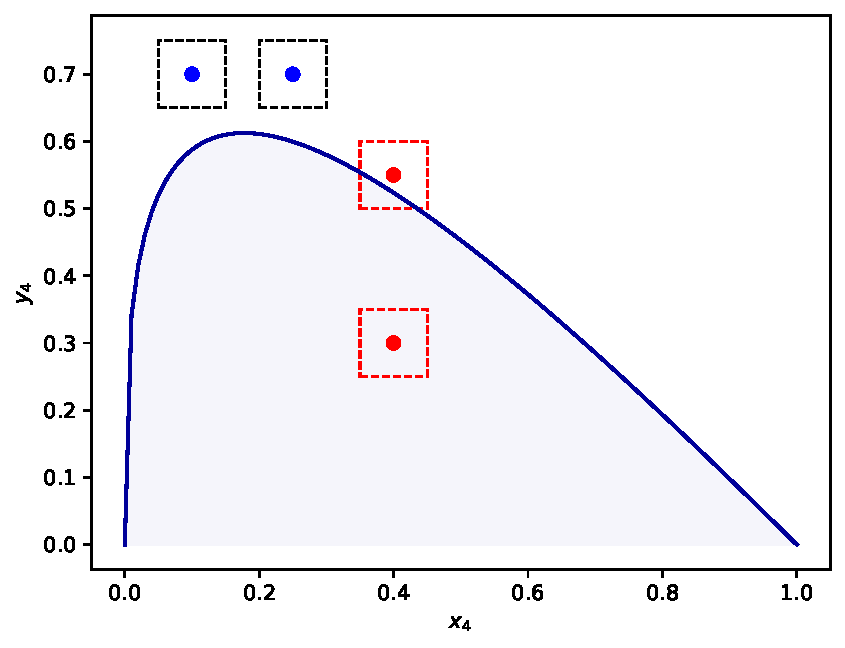
\includegraphics[width = 0.50 \columnwidth]{import/illustrate_lachman_curve.pdf}
  \end{center}
  \caption{
    Illustration of the certification procedure. The blue line represents the Lachman curve $\mathcal{L}_{4}$. States with $y_{4} > \mathcal{L}_{4}(x_{4})$ are genuine Fock states $\ket{4}$. Four example states are depicted in the figure. The bullet points represent their expectation values $\expvalue{x_{4}}$ and $\expvalue{y_{4}}$ obtained by simulating the experiment. The dashed boxes would normally span three standard deviations in each dimension. Size of the pictured boxes are extremely exaggerated for legibility. States marked with red bullets failed the certification as they lie either under the Lachman curve or their respective boxes intersect the curve. States marked with blue bullets are certifiably genuine $4$-photon states according to the criteria; their boxes are well above the curve and do not intersect the curve.
  }
  \label{f-otm-il}
\end{figure}

% Monte Carlo Simulation
%
%

\section{Monte Carlo simulation of the experimental state preparation circuit}

Yadda. Yadda. Yadda.

% Results
%
%

\FloatBarrier
\section{Discussion of results}

In each dataset related to the tuple $(m, \zeta_{1}, \zeta_{2})$ of parameters the maximal probability of success is found with respect to the squeezing rate ${r \leq 10\,\dB}$. Both the maximal probability $P_{m}^{\star}$ and the respective optimal squeezing rate ${r^{\star}}$ are visualised in a grid as functions of ${(1 - \zeta_{1}, 1 - \zeta_{2})}$ for each target state $m$. In addition, to present only statistically significant results in the visualisation, grid cells where the probability of success lies below a reasonable threshold set to $10^{-5}$, which guarantees at least $1000$ successful realizations of the state within each experimental run, were blanked out.

The achievable success rate in preparation and subsequent certification of genuine $m$-photon states is presented in~\figref{f-otm-234}. Each column pertains to the particular target state $m = 2, 3, 4$. The maximal probabilities of success $P_{m}^{\star} (1 - \zeta_{1}, 1 - \zeta_{2})$ are presented in the top row, whereas the corresponding optimal squeezing rates $r^{\star} (1 - \zeta_{1}, 1 - \zeta_{2})$ are provided in the bottom row.
To reflect on the experimental limitations, the optimization is constrained to squeezing rates limited by $10\,\dB$. The figure also effectively shows the amount of loss that can be tolerated in the experiment.

In the case of the $2$-photonic state the tolerable loss exceeds $40\%$ in both modes. The probability of success ranges from roughly $10\%$ to $0.1\%$. The higher the loss, the lower the optimal squeezing rate. The tolerable loss is much lower for the state with $3$ photons. The maximal probabilities of success are also reduced. If the state suffers $40\%$ loss during preparation, it can only tolerate at most $20\%$ loss in its characterization. Higher loss leads to success rates lower than the $10^{-5}$ threshold  set earlier; the information obtained in the blanked out region is assumed to be unreliable. Finally, the conditions for the 4 photon state are even less favorable; while it is still possible to tolerate up to $40\%$ loss during preparation, the limit on $1 - \zeta_{2}$ is much more stringent, only about $10\%$ loss is permitted.

The two mode squeezed vacuum state is assumed to be ideal. The photon number resolving detectors are also presumed to be perfect with unit quantum efficiency. In realistic experiments these assumptions are never true, however, both the inefficiencies in detection and preparation of the squeezed state can be modeled with loss. Consequently the presented results cover these imperfect cases as well since any loss in the initial squeezed state generation are subsumed in the detection losses.

\begin{figure}[h]
  \begin{center}
    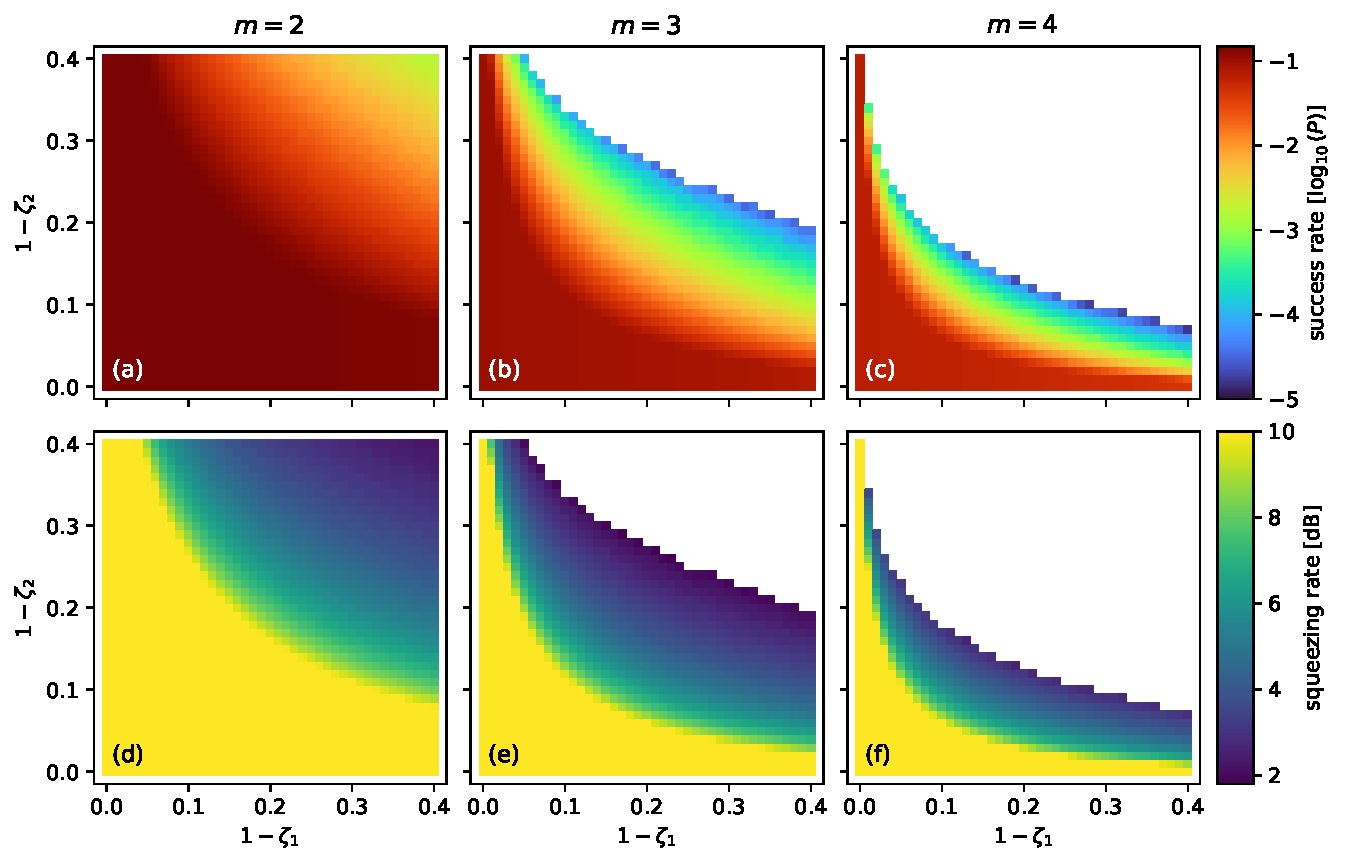
\includegraphics[width = \columnwidth]{import/hierarchy_2-3-4_1000.pdf}
  \end{center}
  \caption{
    The tolerable loss in preparation and subsequent certification of genuine $m$-photon states. Results for target states $m = 2, 3, 4$ are shown in columns. The maximal probabilities $P_{m}^{\star}$ of successful preparation of the certifiable target state, given the particular combination of loss $1 - \zeta_{1}$ incurred during preparation and the loss $1 - \zeta_{2}$ affecting the certification, are presented using a logarithmic scale in the top row. The optimization is constrained to squeezing rates limited by $10\,\dB$. The respective optimal squeezing rates $r^{\star}$ are provided in the bottom row.
  }
  \label{f-otm-234}
\end{figure}

% Conclusions
%
%

\FloatBarrier
\section{Conclusions}

The results presented in this chapter offer an insight into feasible experimental preparation of certifiable genuine $m$-photon states for $m = 2, 3, 4$. While preparation of quantum states of travelling light of up to three photons has already seen its experimental realization~\cite{yukawa2013a}, the construction of a $4$-photon state of travelling light still remains an open problem that will perhaps benefit from the analysis.

% References
%
% 

\FloatBarrier
\printbibliography[heading = bibnumbered]

\end{document}

% vim: linebreak breakindent breakindentopt=shift\:-2 showbreak=↳\  syntax=tex colorcolumn=
